\section{Atmospheric Fit Result Distributions}
\label{sec:fithistos}


%% ATTRIBUTE 0 %%%%%%%%%%%%%%%%%%%%%%%%%%%%%%%%%%%%%%%%%%%%%%%%%%%%%%%%%%%%%%%%%%%
\begin{figure}[h]
  \begin{center}
    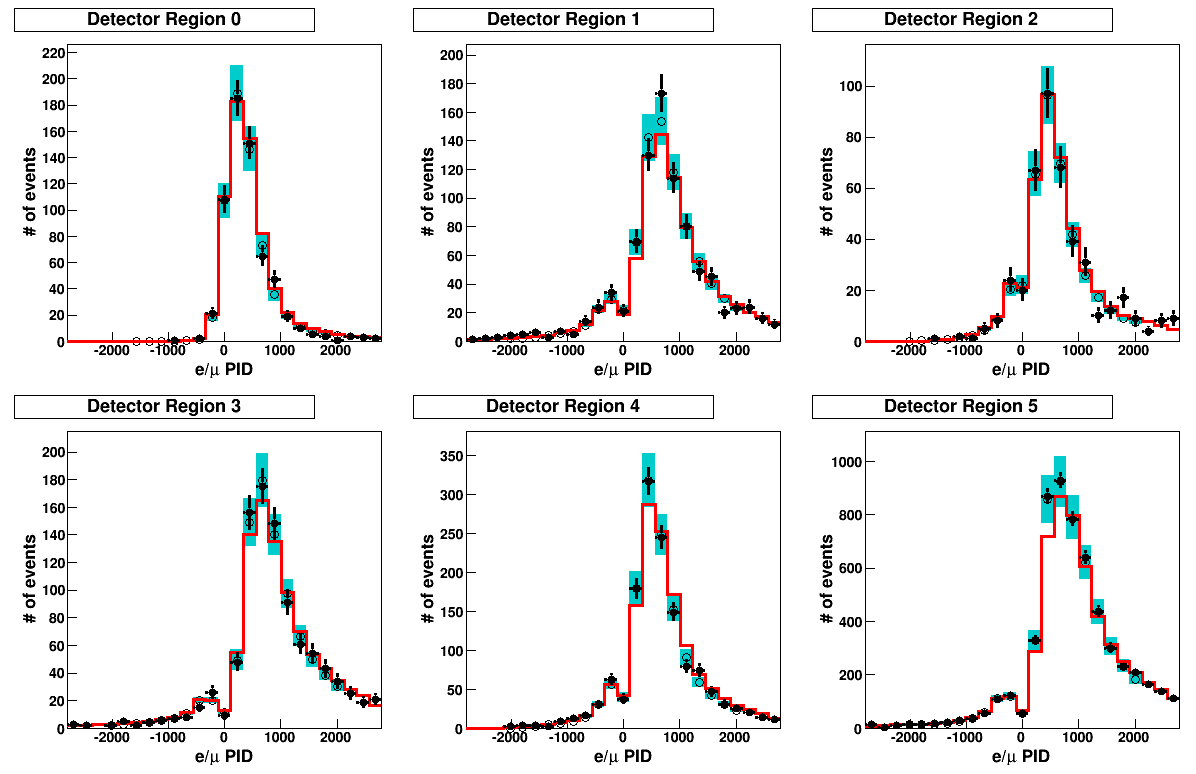
\includegraphics[width=0.9\textwidth]{demcmc_fitresult_samp0_attribute0} 
  \end{center}
  \caption{Fit results for the $l=0$ control sample (no decay electrons) for
  the fiTQun $e/\mu$ PID variable in each of the detector regions.  Positive
  values denote more $e$-like events, negative values denote more $\mu$-like
  events.  Red histogram shows nominal MC prediction.  Black points represent
  observed data.  Teal histogram shows post-fit distribution, where the mean is
  the average of the DE-MCMC throws and the error bar is the square root of the
  variance.}
  \label{fig:fitresults_samp0_att0}
\end{figure}


\begin{figure}[h]
  \begin{center}
    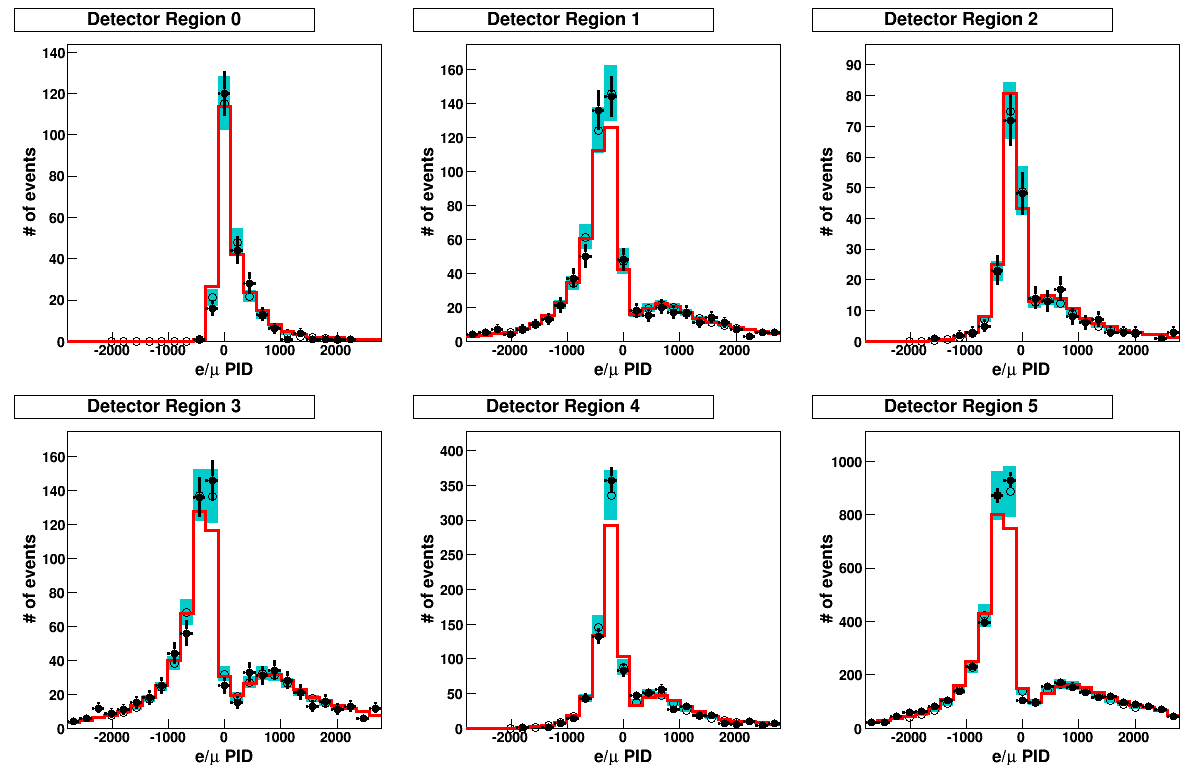
\includegraphics[width=0.9\textwidth]{demcmc_fitresult_samp1_attribute0} 
  \end{center}
  \caption{Fit results for the $l=1$ control sample (one decay electron) for
  the fiTQun $e/\mu$ PID variable in each of the detector regions.  Positive
  values denote more $e$-like events, negative values denote more $\mu$-like
  events.  Red histogram shows nominal MC prediction.  Black points represent
  observed data.  Teal histogram shows post-fit distribution, where the mean is
  the average of the DE-MCMC throws and the error bar is the square root of the
  variance.}
  \label{fig:fitresults_samp1_att0}
\end{figure}


\begin{figure}[h]
  \begin{center}
    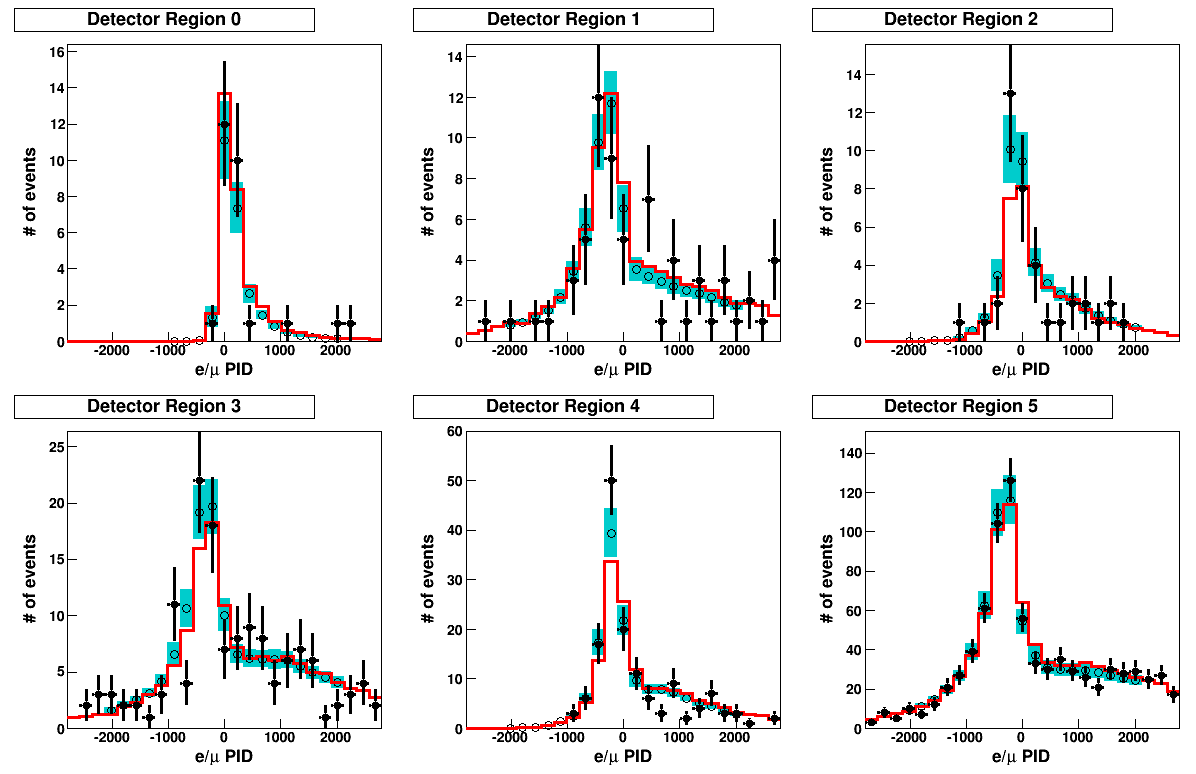
\includegraphics[width=0.9\textwidth]{demcmc_fitresult_samp2_attribute0} 
  \end{center}
  \caption{Fit results for the $l=2$ control sample (more than one decay
  electron) for the fiTQun $e/\mu$ PID variable in each of the detector
  regions.  Positive values denote more $e$-like events, negative values denote
  more $\mu$-like events. Red histogram shows nominal MC prediction.  Black
  points represent observed data.  Teal histogram shows post-fit distribution,
  where the mean is the average of the DE-MCMC throws and the error bar is the
  square root of the variance.}
  \label{fig:fitresults_samp2_att0}
\end{figure}


%% ATTRIBUTE 1 %%%%%%%%%%%%%%%%%%%%%%%%%%%%%%%%%%%%%%%%%%%%%%%%%%%%%%%%%%%%%%%%%%%
\begin{figure}[h]
  \begin{center}
    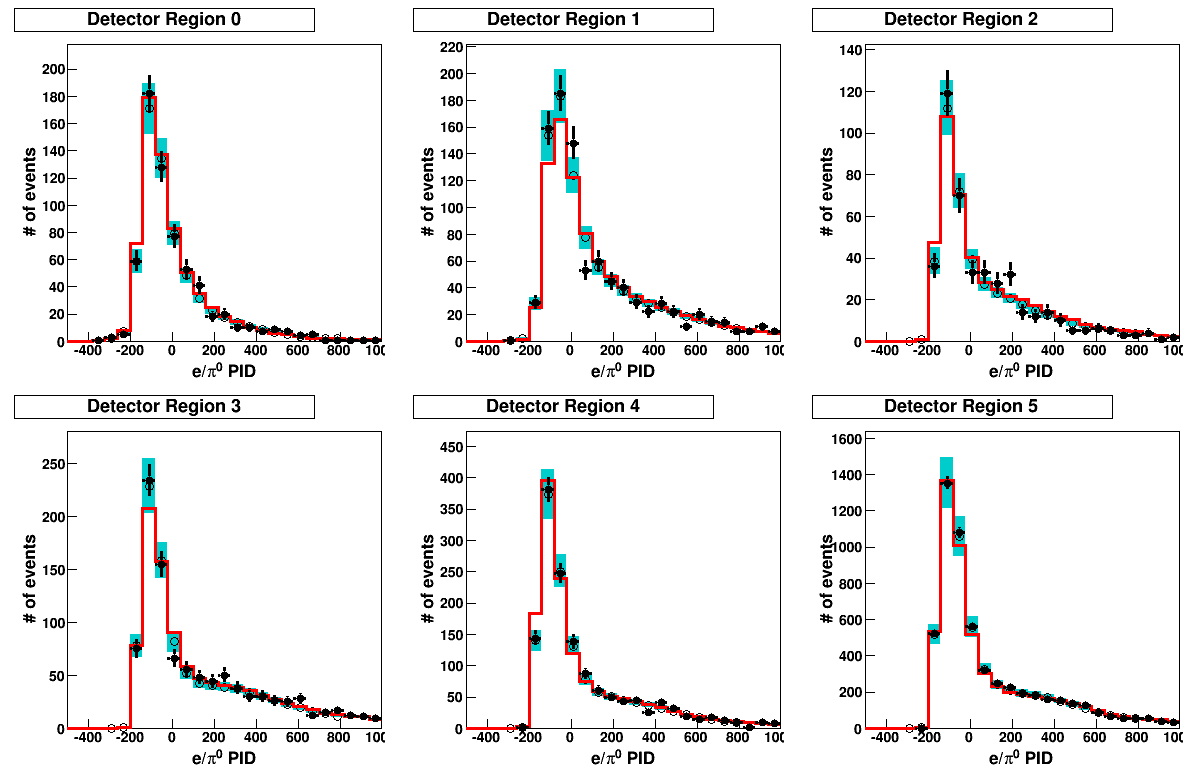
\includegraphics[width=0.9\textwidth]{demcmc_fitresult_samp0_attribute1} 
  \end{center}
  \caption{Fit results for the $l=0$ control sample (no decay electrons) for
  the fiTQun $e/\pi^{0}$ PID variable in each of the detector regions. Positive
  values denote more $\pi^{0}$-like events, negative values denote more
  $e$-like events. Red histogram shows nominal MC prediction.  Black points
  represent observed data.  Teal histogram shows post-fit distribution, where
  the mean is the average of the DE-MCMC throws and the error bar is the square
  root of the variance.}
  \label{fig:fitresults_samp0_att1}
\end{figure}


\begin{figure}[h]
  \begin{center}
    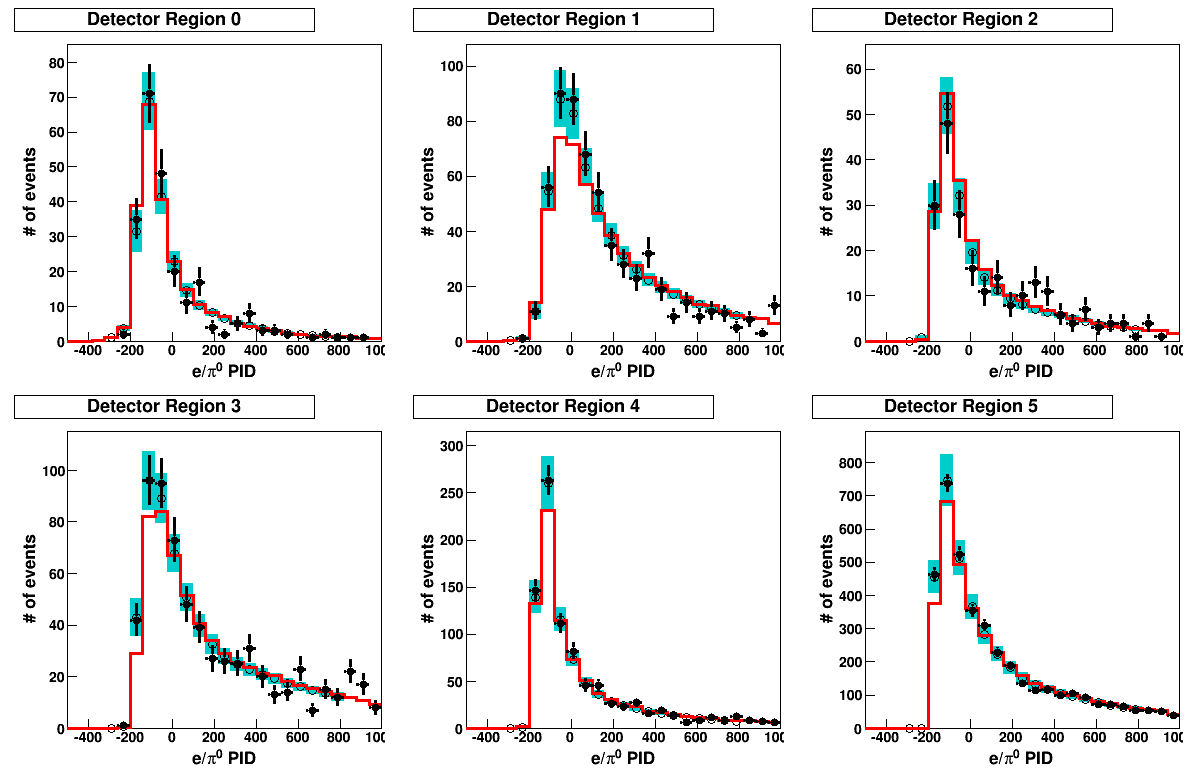
\includegraphics[width=0.9\textwidth]{demcmc_fitresult_samp1_attribute1} 
  \end{center}
  \caption{Fit results for the $l=1$ control sample (one decay electron) for
  the fiTQun $e/\pi^{0}$ PID variable in each of the detector regions. Positive
  values denote more $\pi^{0}$-like events, negative values denote more
  $e$-like events. Red histogram shows nominal MC prediction.  Black points
  represent observed data.  Teal histogram shows post-fit distribution, where
  the mean is the average of the DE-MCMC throws and the error bar is the square
  root of the variance.}
  \label{fig:fitresults_samp1_att1}
\end{figure}


\begin{figure}[h]
  \begin{center}
    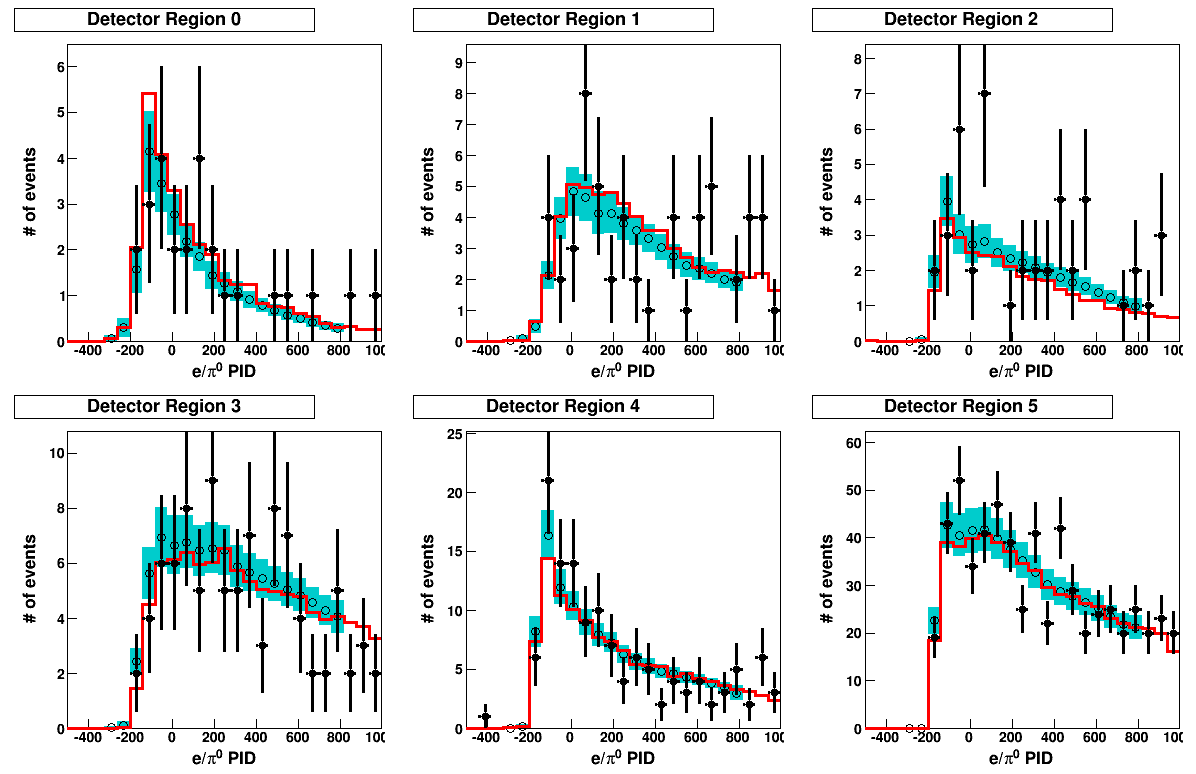
\includegraphics[width=0.9\textwidth]{demcmc_fitresult_samp2_attribute1} 
  \end{center}
  \caption{Fit results for the $l=2$ control sample (more than one decay
  electron) for the fiTQun $e/\pi^{0}$ PID variable in each of the detector
  regions.  Positive values denote more $\pi^{0}$-like events, negative values
  denote more $e$-like events. Red histogram shows nominal MC prediction.
  Black points represent observed data.  Teal histogram shows post-fit
  distribution, where the mean is the average of the DE-MCMC throws and the
  error bar is the square root of the variance.}
  \label{fig:fitresults_samp2_att1}
\end{figure}


%% ATTRIBUTE 2 %%%%%%%%%%%%%%%%%%%%%%%%%%%%%%%%%%%%%%%%%%%%%%%%%%%%%%%%%%%%%%%%%%%
\begin{figure}[h]
  \begin{center}
    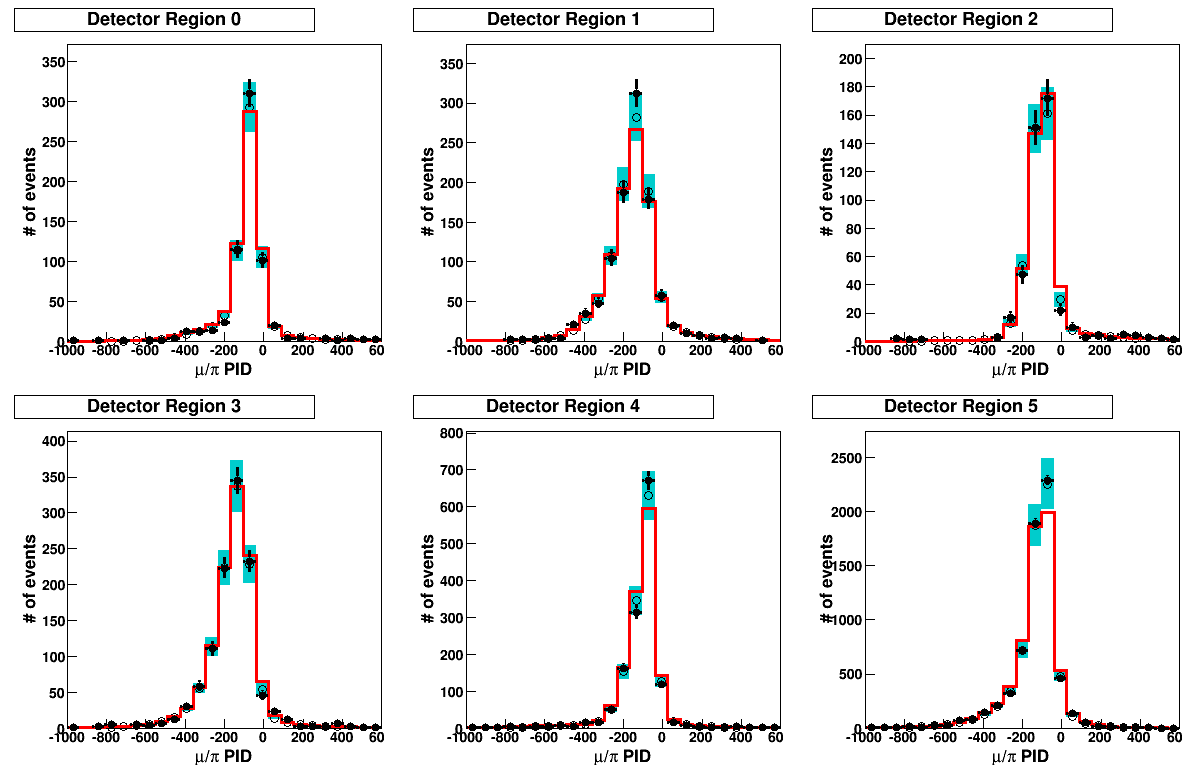
\includegraphics[width=0.9\textwidth]{demcmc_fitresult_samp0_attribute2} 
  \end{center}
  \caption{Fit results for the $l=0$ control sample (no decay electrons) for
  the fiTQun $\mu/\pi$ PID variable in each of the detector regions. Positive
  values denote more $\pi$-like events, negative values denote more $\mu$-like
  events. Red histogram shows nominal MC prediction.  Black points represent
  observed data.  Teal histogram shows post-fit distribution, where the mean is
  the average of the DE-MCMC throws and the error bar is the square root of the
  variance.}
  \label{fig:fitresults_samp0_att2}
\end{figure}


\begin{figure}[h]
  \begin{center}
    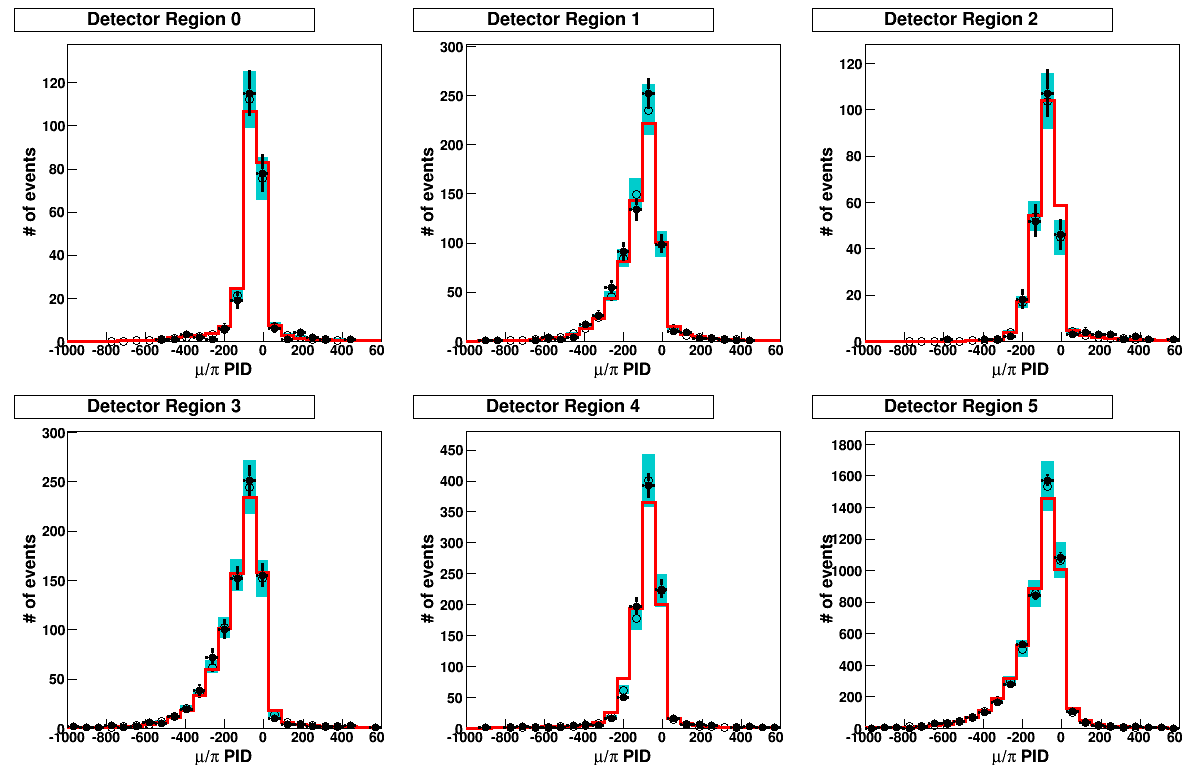
\includegraphics[width=0.9\textwidth]{demcmc_fitresult_samp1_attribute2} 
  \end{center}
  \caption{Fit results for the $l=1$ control sample (one decay electron) for
  the fiTQun $\mu/\pi$ PID variable in each of the detector regions.  Positive
  values denote more $\pi$-like events, negative values denote more $\mu$-like
  events. Red histogram shows nominal MC prediction.  Black points represent
  observed data.  Teal histogram shows post-fit distribution, where the mean is
  the average of the DE-MCMC throws and the error bar is the square root of the
  variance.} 
  \label{fig:fitresults_samp1_att2}
\end{figure}


\begin{figure}[h]
  \begin{center}
    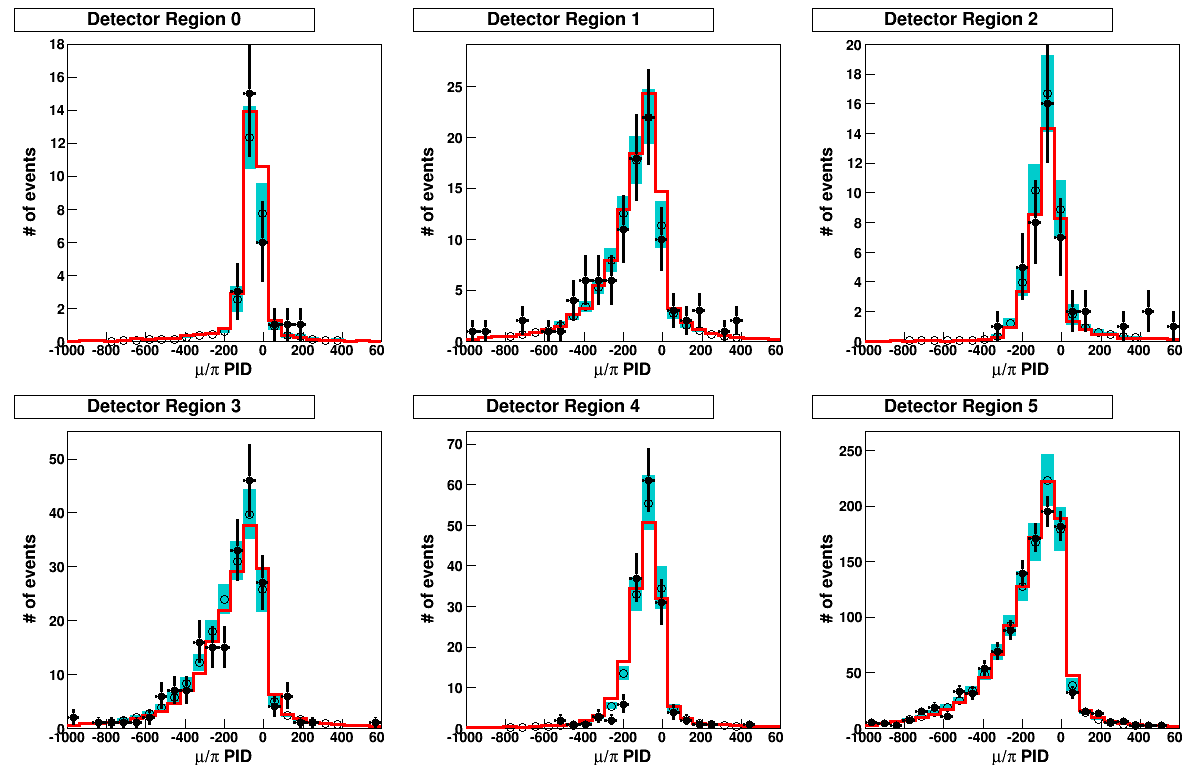
\includegraphics[width=0.9\textwidth]{demcmc_fitresult_samp2_attribute2} 
  \end{center}
  \caption{Fit results for the $l=2$ control sample (more than one decay
  electron) for the fiTQun $\mu/\pi$ PID variable in each of the detector
  regions.  Positive values denote more $\pi$-like events, negative values
  denote more $\mu$-like events. Red histogram shows nominal MC prediction.
  Black points represent observed data.  Teal histogram shows post-fit
  distribution, where the mean is the average of the DE-MCMC throws and the
  error bar is the square root of the variance.}
  \label{fig:fitresults_samp2_att2}
\end{figure}


%% ATTRIBUTE 3 %%%%%%%%%%%%%%%%%%%%%%%%%%%%%%%%%%%%%%%%%%%%%%%%%%%%%%%%%%%%%%%%%%%
\begin{figure}[h]
  \begin{center}
    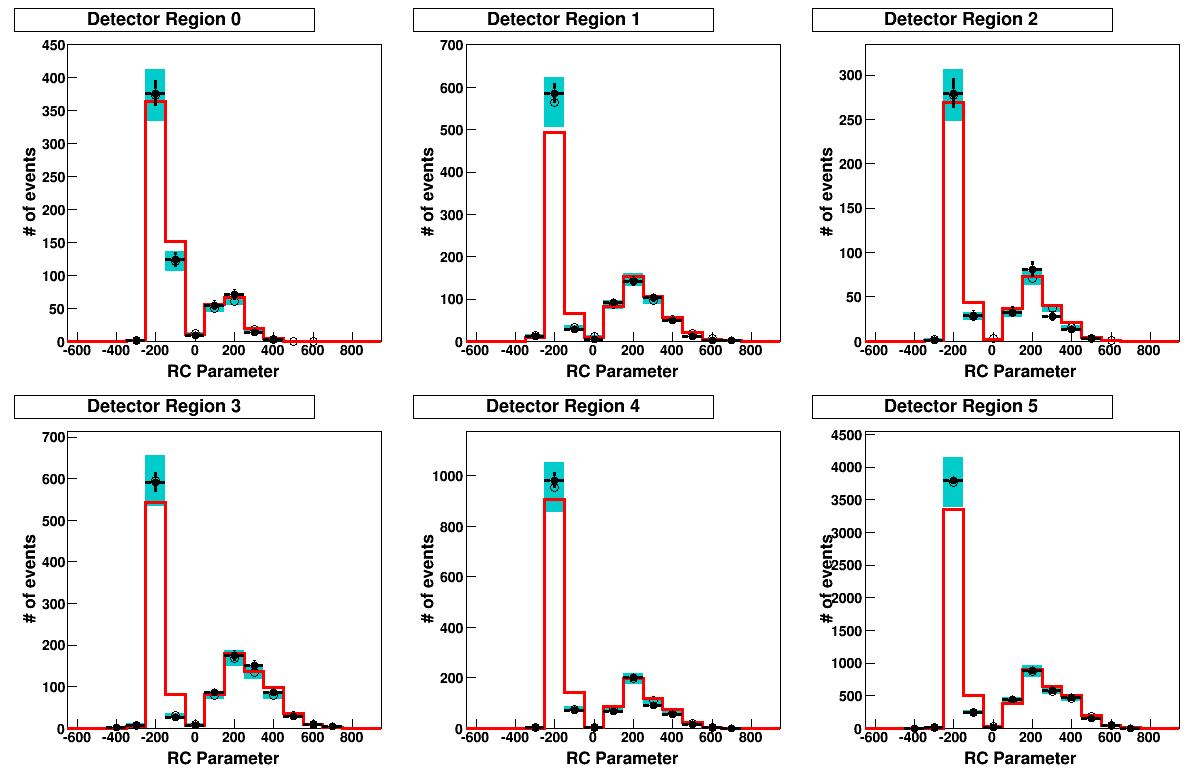
\includegraphics[width=0.9\textwidth]{demcmc_fitresult_samp0_attribute3} 
  \end{center}
  \caption{Fit results for the $l=0$ control sample (no decay electrons) for
  the fiTQun RC (ring-counting) variable in each of the detector regions.
  Positive values denote more multi-ring-like events, negative values denote
  more single-ring-like events. Red histogram shows nominal MC prediction.
  Black points represent observed data.  Teal histogram shows post-fit
  distribution, where the mean is the average of the DE-MCMC throws and the
  error bar is the square root of the variance.}
  \label{fig:fitresults_samp0_att3}
\end{figure}


\begin{figure}[h]
  \begin{center}
    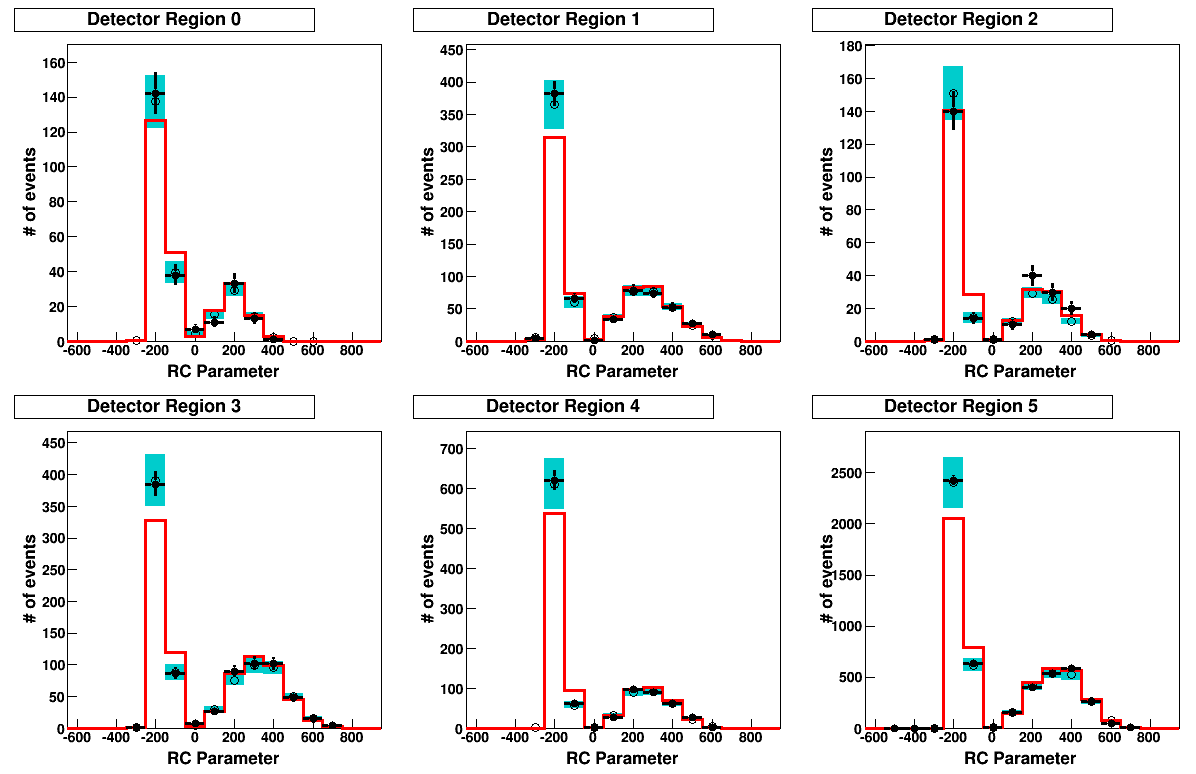
\includegraphics[width=0.9\textwidth]{demcmc_fitresult_samp1_attribute3} 
  \end{center}
  \caption{Fit results for the $l=1$ control sample (one decay electron) for
  the fiTQun $\mu/\pi$ PID variable in each of the detector regions.  Positive
  values denote more multi-ring-like events, negative values denote more
  single-ring-like events. Red histogram shows nominal MC prediction.  Black
  points represent observed data.  Teal histogram shows post-fit distribution,
  where the mean is the average of the DE-MCMC throws and the error bar is the
  square root of the variance.}
  \label{fig:fitresults_samp1_att3}
\end{figure}


\begin{figure}[h]
  \begin{center}
    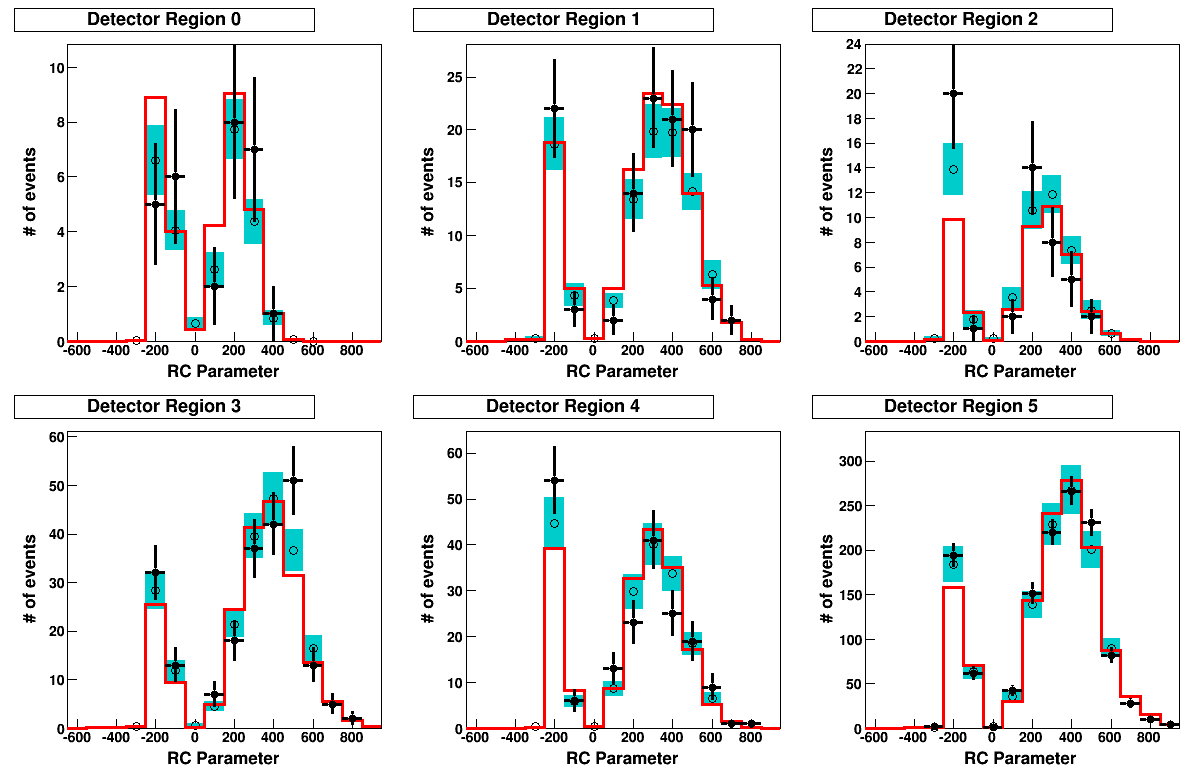
\includegraphics[width=0.9\textwidth]{demcmc_fitresult_samp2_attribute3} 
  \end{center}
  \caption{Fit results for the $l=2$ control sample (more than one decay
  electron) for the fiTQun $\mu/\pi$ PID variable in each of the detector
  regions.  Positive values denote more multi-ring-like events, negative values
  denote more single-ring-like events.  Red histogram shows nominal MC
  prediction.  Black points represent observed data.  Teal histogram shows
  post-fit distribution, where the mean is the average of the DE-MCMC throws
  and the error bar is the square root of the variance.}
  \label{fig:fitresults_samp2_att3}
\end{figure}

